\documentclass[a4paper,12pt]{article}
\usepackage{amsmath}
\usepackage{amssymb}
\usepackage[polish]{babel}
\usepackage{polski}
\usepackage[utf8]{inputenc}
\usepackage{indentfirst}
\usepackage{geometry}
\usepackage{array}
\usepackage[pdftex]{color,graphicx}
\usepackage{subfigure}
\usepackage{afterpage}
\usepackage{setspace}
\usepackage{color}
\usepackage{wrapfig}
\usepackage{listings}
\usepackage{datetime}
\usepackage[outdir=./]{epstopdf}

\renewcommand{\onehalfspacing}{\setstretch{1.6}}

\geometry{tmargin=2.5cm,bmargin=2.5cm,lmargin=2.5cm,rmargin=2.5cm}
\setlength{\parindent}{1cm}
\setlength{\parskip}{0mm}

\newenvironment{lista}{
\begin{itemize}
  \setlength{\itemsep}{1pt}
  \setlength{\parskip}{0pt}
  \setlength{\parsep}{0pt}
}{\end{itemize}}

\newcommand{\linia}{\rule{\linewidth}{0.4mm}}

\definecolor{lbcolor}{rgb}{0.95,0.95,0.95}
\lstset{
    backgroundcolor=\color{lbcolor},
    tabsize=4,
  language=C++,
  captionpos=b,
  tabsize=3,
  frame=lines,
  numbers=left,
  numberstyle=\tiny,
  numbersep=5pt,
  breaklines=true,
  showstringspaces=false,
  basicstyle=\footnotesize,
  identifierstyle=\color{magenta},
  keywordstyle=\color[rgb]{0,0,1},
  commentstyle=\color{Darkgreen},
  stringstyle=\color{red}
  }

\begin{document}

\noindent
\begin{tabular}{|c|p{11cm}|c|} \hline 
Grupa 1 & Kordian Kurdziel, Mateusz Maciejak & \ddmmyyyydate\today \tabularnewline
\hline 
\end{tabular}


\section*{Zadanie 5 - Liczby pierwsze - MPI}

Celem programu był test czy liczby podane w pliku są liczbami pierwszymi. W celu poprawy wydajności programu do zrównoleglenia jego działania należało wykorzystać standard MPI.
Program przyjmuje dwa argumenty, obraz wejściowy oraz obraz wyjściowy. Liczbę procesów na jakich mają zostać wykoanane obliczenia należy podać po komendzie mpirun używając flagi -n.

Do komunikacji między procesami wykorzystane zostały funkcje standardu MPI - MPI\_Send i MPI\_Recv. Na poniższym listingu można zobaczyć ich sygnaturę.

\begin{lstlisting}
  MPI_Send(
      void* data,
      int count,
      MPI_Datatype datatype,
      int destination,
      int tag,
      MPI_Comm communicator)
  MPI_Recv(
      void* data,
      int count,
      MPI_Datatype datatype,
      int source,
      int tag,
      MPI_Comm communicator,
      MPI_Status* status)
\end{lstlisting}

Poniższy listing przedstawia algorytm wyznaczania liczby pierwszej. Został wybrany algorytm naiwny, ponieważ gwarantował poprawność wyników, a ilość i długość testowanych liczb nie była na tyle długa by powodowało to znaczące obniżenie wydajności obliczeń. 
W poszczególnych wątkach sprawdzane jest czy dana liczba jest liczbą pierwszą. Dane zostają podzielone na części i obliczane równolegle, używając wewnętrznych kopii danych w procesie.

\begin{lstlisting}
bool isPrime(ll n)
{
    if(n<2)
        return false;
        
    for(ll i=2;i*i<=n;i++)
        if(n%i==0)
            return false; 

    return true;
}

\end{lstlisting}



Poniższe wykresy 1 i 2, przedstawiające zależność czasową oraz przyspieszenia zostały oparte na średnich wynikach programu uruchamianych lokalnie na maszynie wirtualnej. Wykorzystany został 6 rdzeniowy procesor Intel i7-8700K z technologią Hyperthreadingu.

\begin{figure}[!ht]
	\centering
  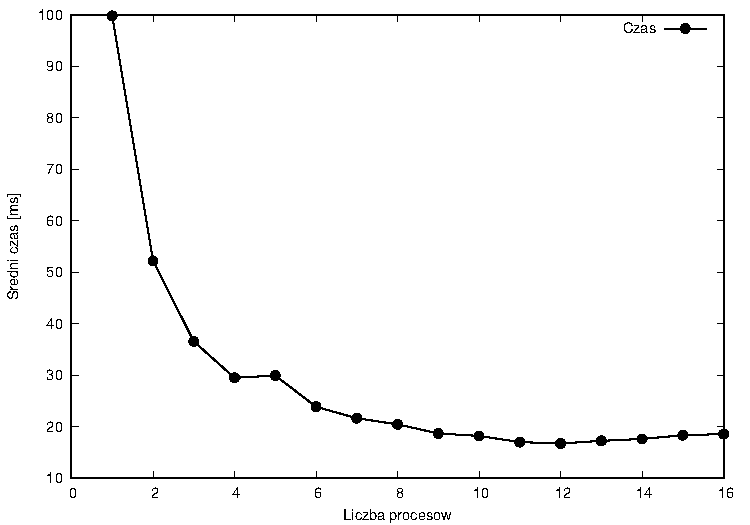
\includegraphics[width=0.7\textwidth]{wykresCzas.pdf}
  \caption{Wykres zależności czasu wykonywania obliczeń od liczby procesów}
\end{figure}

\begin{figure}[!ht]
	\centering
  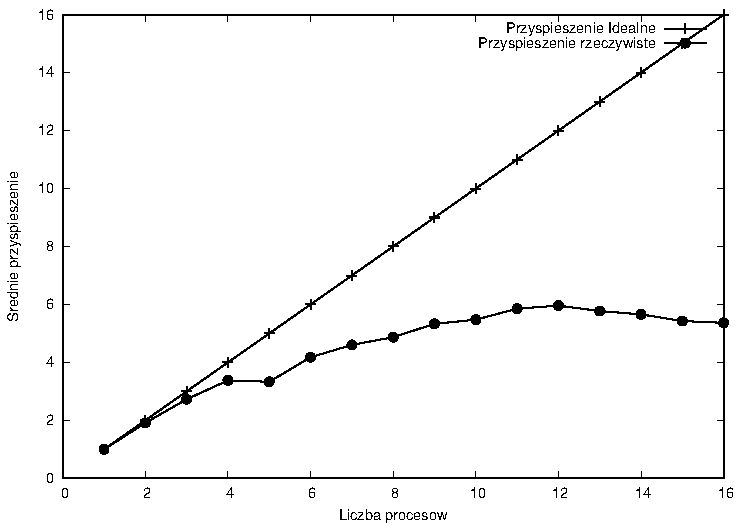
\includegraphics[width=0.7\textwidth]{wykresPrzyspieszenie.pdf}
  \caption{Wykres przyspieszenia działania programu w zależności od liczby procesów}
\end{figure}


Jak widać dzięki zastosowaniu technologii MPI, wykorzystując dostępne procesy, udało się znacząco przyspieszyć wykonywanie programu. Uzyskane rzeczywiste przyspieszenie jest bliskie idealnemu, co może świadczyć o tym, że powyższa klasa problemów nadaje się całkiem dobrze do wykorzystywania obliczeń wielowątkowych.
Na podstawie otrzymanych wyników można stwierdzić, że technologia Hyperthreadingu pomogła przyspieszyć obliczenia. Wirtualne rdzenie nie pozwalały przyspieszyć obliczenia równie sprawnie jak te rzeczywiste, ale czasy uzyskane z ich wykorzystaniem są znacząco niższe niż te bez ich użycia.

\end{document}
